\documentclass[a4paper,12pt]{article}
\usepackage[utf8]{inputenc}
\usepackage[T1]{fontenc}
\usepackage[margin=1in]{geometry}
\usepackage{amsmath, amssymb, mathtools}
\usepackage[version=4]{mhchem}
\usepackage{tcolorbox}
\usepackage{enumitem}
\usepackage{fancyhdr}
\usepackage{titlesec}
\usepackage{tikz}
\usepackage{pgfplots}
\usepackage{hyperref}
\usepackage{longtable}
\usepackage{array}
\usepackage{float}

\usetikzlibrary{patterns, decorations.pathmorphing, decorations.markings, arrows.meta}
\pgfplotsset{compat=1.18}

% Header and Footer
\pagestyle{fancy}
\fancyhf{}
\fancyhead[L]{Engineering Chemistry (DI01000071)}
\fancyhead[R]{Winter 2024 Solution}
\fancyfoot[C]{\thepage}

% Title Formatting
\titleformat{\section}{\large\bfseries}{\thesection}{1em}{}
\titleformat{\subsection}{\bfseries}{\thesubsection}{1em}{}

% Custom Environments
\newtcolorbox{solutionbox}{
    colback=gray!5,
    colframe=gray!40,
    boxrule=0.5pt,
    arc=2pt,
    left=5pt, right=5pt, top=5pt, bottom=5pt
}

\begin{document}

\begin{center}
    {\Large\textbf{Engineering Chemistry (DI01000071) - Winter 2024 Solution}}\\[0.5cm]
    \textit{Date: 2025-01-09}
\end{center}

\section*{Question 1 [14 marks]}
\textbf{Fill in the blanks using appropriate choice from the given options:}

\begin{solutionbox}
\textbf{Answer}:

\begin{longtable}{|p{0.8cm}|p{2.5cm}|p{10cm}|}
\hline
(1) & \ce{[Ar]4s^1 3d^10} & Cu has 29 electrons, exception to Aufbau rule \\ \hline
(2) & 14 & pH + pOH = 14 at $25^\circ$C \\ \hline
(3) & cathode & Pure copper deposits at negative electrode \\ \hline
(4) & Cu & Copper forms protective oxide layer \\ \hline
(5) & semi-solid & Peat is partially decomposed organic matter \\ \hline
(6) & Dulong & Dulong's formula calculates calorific value \\ \hline
(7) & Lignite & Lignite has highest moisture (35-75\%) \\ \hline
(8) & Poise & SI unit of dynamic viscosity \\ \hline
(9) & High & High flash point prevents ignition \\ \hline
(10) & Emulsion & Oil-water mixture forms emulsion \\ \hline
(11) & Bakelite & Phenol formaldehyde = Bakelite \\ \hline
(12) & S & Sulfur used for vulcanization \\ \hline
(13) & PHBV & PHBV is biodegradable polymer \\ \hline
(14) & volt & EMF measured in volts \\ \hline
\end{longtable}

\textbf{Mnemonic:} "Chemical Copper Creates Beautiful Properties" (for remembering key concepts)
\end{solutionbox}

\section*{Question 2(A) [6 marks]}

\subsection*{Question 2(A)(1) [3 marks]}
\textbf{List the three importance of pH in various fields.}

\begin{solutionbox}
\textbf{Answer}:

\begin{tabular}{|l|l|l|}
\hline
\textbf{Field} & \textbf{Importance} & \textbf{Application} \\ \hline
\textbf{Medicine} & Blood pH maintenance & Normal pH 7.35-7.45 for proper body function \\ \hline
\textbf{Agriculture} & Soil pH optimization & pH 6-7 ideal for crop growth and nutrient absorption \\ \hline
\textbf{Industry} & Quality control & pH affects product quality in food, textiles, pharmaceuticals \\ \hline
\end{tabular}

\textbf{Mnemonic:} "Medical Agriculture Industry" (MAI)
\end{solutionbox}

\subsection*{Question 2(A)(2) [3 marks]}
\textbf{Define: Buffer solutions, Half-cell, Faraday's first law of electrolysis.}

\begin{solutionbox}
\textbf{Answer}:
\begin{itemize}
    \item \textbf{Buffer solutions}: Solutions that resist changes in pH when small amounts of acid or base are added.
    \item \textbf{Half-cell}: Single electrode immersed in its ionic solution, represents oxidation or reduction reaction.
    \item \textbf{Faraday's first law}: Amount of substance deposited/liberated at electrode is directly proportional to quantity of electricity passed ($w \propto Q$).
\end{itemize}
\textbf{Mnemonic:} "Buffers Help Faraday" (BHF)
\end{solutionbox}

\subsection*{Question 2(A)(3) [3 marks]}
\textbf{State the factors affecting the rate of corrosion.}

\begin{solutionbox}
\textbf{Answer}:
\begin{tabular}{|l|l|l|}
\hline
\textbf{Factor} & \textbf{Effect} & \textbf{Description} \\ \hline
\textbf{Metal purity} & Higher purity = Less corrosion & Impurities create galvanic cells \\ \hline
\textbf{Temperature} & Higher temp = Faster corrosion & Increases reaction rate \\ \hline
\textbf{Humidity} & Higher humidity = More corrosion & Promotes electrochemical reactions \\ \hline
\end{tabular}

\textbf{Mnemonic:} "Pure Temperature Humidity" (PTH)
\end{solutionbox}

\section*{Question 2(B) [8 marks]}

\subsection*{Question 2(B)(1) [4 marks]}
\textbf{Compare between orbits and orbitals (four points each).}

\begin{solutionbox}
\textbf{Answer}:
\begin{tabular}{|l|p{5cm}|p{5cm}|}
\hline
\textbf{Aspect} & \textbf{Orbits} & \textbf{Orbitals} \\ \hline
\textbf{Definition} & Fixed circular paths & 3D probability regions \\ \hline
\textbf{Shape} & Circular/elliptical & s, p, d, f shapes \\ \hline
\textbf{Energy} & Definite energy levels & Energy ranges \\ \hline
\textbf{Electron location} & Exact position & Probability of finding \\ \hline
\end{tabular}

\vspace{0.5cm}
\textbf{Diagram:}
\begin{center}
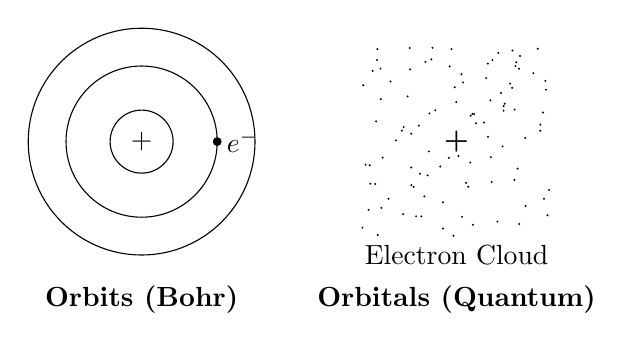
\begin{tikzpicture}[scale=0.8]
    % Bohr Model
    \node at (0, -2.5) {\textbf{Orbits (Bohr)}};
    \draw (0,0) circle (0.5); \node at (0,0) {+};
    \draw (0,0) circle (1.2); \fill (1.2,0) circle (2pt) node[right] {$e^-$};
    \draw (0,0) circle (1.8);
    
    % Quantum Model
    \begin{scope}[xshift=5cm]
        \node at (0, -2.5) {\textbf{Orbitals (Quantum)}};
        \foreach \i in {1,...,100} \fill (rand*1.5, rand*1.5) circle (0.5pt);
        \node at (0,0) {\textbf{+}};
        \node at (0,-1.8) {Electron Cloud};
    \end{scope}
\end{tikzpicture}
\end{center}

\textbf{Mnemonic:} "Definite Shape Energy Location" (DSEL)
\end{solutionbox}

\subsection*{Question 2(B)(2) [4 marks]}
\textbf{Classify fuels on the basis of its sources and physical states with one example of each.}

\begin{solutionbox}
\textbf{Answer}:
\begin{tabular}{|l|l|l|l|}
\hline
\textbf{Classification} & \textbf{Type} & \textbf{Example} & \textbf{Description} \\ \hline
\textbf{Source-based} & Natural & Coal & Formed naturally \\ \hline
 & Artificial & Petrol & Man-made \\ \hline
\textbf{Physical state} & Solid & Wood & Solid at room temp \\ \hline
 & Liquid & Diesel & Liquid at room temp \\ \hline
 & Gaseous & LPG & Gas at room temp \\ \hline
\end{tabular}

\textbf{Mnemonic:} "Natural Artificial, Solid Liquid Gas" (NASLG)
\end{solutionbox}

\subsection*{Question 2(B)(3) [4 marks]}
\textbf{Explain bio-diesel with four important points.}

\begin{solutionbox}
\textbf{Answer}:
\begin{itemize}
    \item \textbf{Source}: Made from vegetable oils, animal fats, or waste cooking oil.
    \item \textbf{Process}: Produced by transesterification reaction with methanol/ethanol.
    \item \textbf{Properties}: Biodegradable, non-toxic, renewable fuel source.
    \item \textbf{Applications}: Used in diesel engines, reduces emissions by 75\%.
\end{itemize}

\textbf{Chemical Reaction:}
\[ \text{Vegetable Oil} + \text{Methanol} \xrightarrow{\text{Catalyst}} \text{Bio-diesel} + \text{Glycerol} \]

\textbf{Mnemonic:} "Source Process Properties Applications" (SPPA)
\end{solutionbox}

\section*{Question 3(A) [6 marks]}

\subsection*{Question 3(A)(1) [3 marks]}
\textbf{Explain solute, solvent and solution with the help of example.}

\begin{solutionbox}
\textbf{Answer}:
\begin{tabular}{|l|l|l|}
\hline
\textbf{Component} & \textbf{Definition} & \textbf{Example} \\ \hline
\textbf{Solute} & Substance being dissolved & Salt (\ce{NaCl}) \\ \hline
\textbf{Solvent} & Substance doing the dissolving & Water (\ce{H2O}) \\ \hline
\textbf{Solution} & Homogeneous mixture & Salt water \\ \hline
\end{tabular}

\textbf{Example}: Sugar + Water = Sugar solution
\begin{itemize}
    \item Sugar = Solute, Water = Solvent, Sugar water = Solution
\end{itemize}
\textbf{Mnemonic:} "Solute Solvent Solution" (SSS)
\end{solutionbox}

\subsection*{Question 3(A)(2) [3 marks]}
\textbf{Explain the formation of Electrovalent bond in NaCl.}

\begin{solutionbox}
\textbf{Answer}:
\textbf{Process}:
\begin{enumerate}
    \item \textbf{Step 1}: Na loses 1 electron $\to$ \ce{Na^+} (cation)
    \item \textbf{Step 2}: Cl gains 1 electron $\to$ \ce{Cl^-} (anion)
    \item \textbf{Step 3}: Electrostatic attraction between \ce{Na^+} and \ce{Cl^-} forms \ce{NaCl}.
\end{enumerate}

\textbf{Reaction:}
\begin{center}
    \ce{Na -> Na+ + e-} \\
    \ce{Cl + e- -> Cl-} \\
    \ce{Na+ + Cl- -> NaCl}
\end{center}

\textbf{Mnemonic:} "Sodium Loses, Chlorine Gains, Attraction Forms" (SLCGAF)
\end{solutionbox}

\subsection*{Question 3(A)(3) [3 marks]}
\textbf{Explain Octane number for gasoline.}

\begin{solutionbox}
\textbf{Answer}:
\begin{tabular}{|l|l|}
\hline
\textbf{Aspect} & \textbf{Description} \\ \hline
\textbf{Definition} & Measure of fuel's resistance to knocking \\ \hline
\textbf{Scale} & 0-100, higher = better anti-knock properties \\ \hline
\textbf{Standard} & n-heptane = 0, iso-octane = 100 \\ \hline
\end{tabular}
\textbf{Applications}: High octane fuel prevents engine knocking, improves performance.

\textbf{Mnemonic:} "Octane Opposes Knocking" (OOK)
\end{solutionbox}

\section*{Question 3(B) [8 marks]}

\subsection*{Question 3(B)(1) [4 marks]}
\textbf{Explain electrorefining of impure Cu with chemical equations and a labeled diagram.}

\begin{solutionbox}
\textbf{Answer}:
\textbf{Process}:
\begin{itemize}
    \item \textbf{Anode}: Impure copper (Thick rod) - dissolves.
    \item \textbf{Cathode}: Pure copper (Thin strip) - deposits.
    \item \textbf{Electrolyte}: Acidified \ce{CuSO4} solution.
\end{itemize}

\textbf{Chemical Equations}:
\begin{itemize}
    \item At Anode: \ce{Cu -> Cu^2+ + 2e-} (Oxidation)
    \item At Cathode: \ce{Cu^2+ + 2e- -> Cu} (Reduction)
\end{itemize}

\textbf{Diagram:}
\begin{center}
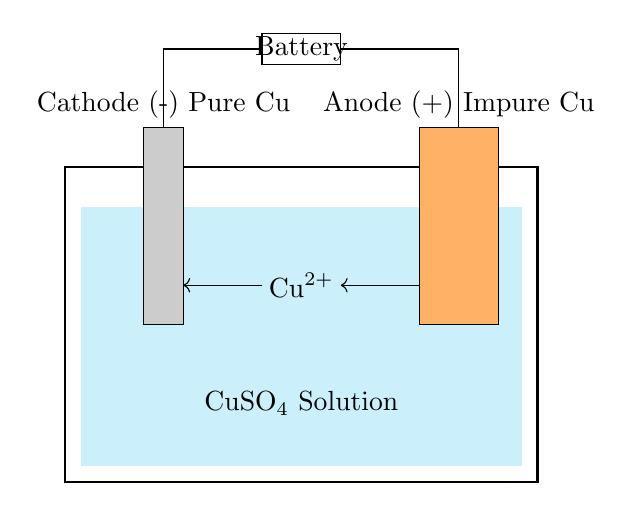
\begin{tikzpicture}
    % Container
    \draw[thick] (0,0) rectangle (6,4);
    \fill[cyan!20] (0.2,0.2) rectangle (5.8,3.5);
    \node at (3,1) {\ce{CuSO4} Solution};
    
    % Electrodes
    \draw[fill=gray!40] (1,2) rectangle (1.5,4.5); \node at (1.25, 4.8) {Cathode (-) Pure Cu};
    \draw[fill=orange!60] (4.5,2) rectangle (5.5,4.5); \node at (5, 4.8) {Anode (+) Impure Cu};
    
    % Circuit
    \draw (1.25, 4.5) -- (1.25, 5.5) -- (2.5, 5.5);
    \draw (5, 4.5) -- (5, 5.5) -- (3.5, 5.5);
    \draw (2.5, 5.3) rectangle (3.5, 5.7); \node at (3, 5.5) {Battery};
    
    % Ions
    \node at (3, 2.5) {\ce{Cu^2+}};
    \draw[->] (4.5, 2.5) -- (3.5, 2.5);
    \draw[->] (2.5, 2.5) -- (1.5, 2.5);
\end{tikzpicture}
\end{center}

\textbf{Mnemonic:} "Anode Dissolves, Cathode Deposits" (ADCD)
\end{solutionbox}

\subsection*{Question 3(B)(2) [4 marks]}
\textbf{Explain preparation of ethene with chemical equation. Also write its two properties and two uses.}

\begin{solutionbox}
\textbf{Answer}:
\textbf{Preparation}: Dehydration of ethanol with conc. \ce{H2SO4} at 170$^\circ$C.
\[ \ce{C2H5OH ->[Conc. H2SO4][170^\circ C] C2H4 + H2O} \]

\textbf{Properties}:
\begin{itemize}
    \item \textbf{Physical}: Colorless, sweet-smelling gas.
    \item \textbf{Chemical}: Unsaturated hydrocarbon, undergoes addition reactions.
\end{itemize}

\textbf{Uses}:
\begin{itemize}
    \item Manufacturing polyethylene plastic.
    \item Artificial ripening of fruits.
\end{itemize}

\textbf{Mnemonic:} "Preparation Properties Uses" (PPU)
\end{solutionbox}

\subsection*{Question 3(B)(3) [4 marks]}
\textbf{Explain preparation of Buna-S rubber with chemical equation. Also write its two properties and two uses.}

\begin{solutionbox}
\textbf{Answer}:
\textbf{Preparation}: Copolymerization of 1,3-Butadiene and Styrene in 3:1 ratio.
\[ \ce{n CH2=CH-CH=CH2 + n C6H5-CH=CH2 -> -[CH2-CH=CH-CH2-CH(C6H5)-CH2]_n-} \]
(Butadiene + Styrene $\to$ Buna-S)

\textbf{Properties}:
\begin{itemize}
    \item High abrasion resistance.
    \item High load-bearing capacity.
\end{itemize}

\textbf{Uses}:
\begin{itemize}
    \item Manufacturing automobile tires.
    \item Conveyor belts and hoses.
\end{itemize}

\textbf{Mnemonic:} "Butadiene Styrene Makes Strong Rubber" (BSMSR)
\end{solutionbox}

\section*{Question 4(A) [6 marks]}

\subsection*{Question 4(A)(1) [3 marks]}
\textbf{Explain metal cladding for the prevention of corrosion of metals.}

\begin{solutionbox}
\textbf{Answer}:
\begin{itemize}
    \item \textbf{Process}: Sandwiching the base metal between two layers of corrosion-resistant metal (like Al, Ni).
    \item \textbf{Method}: Sheets of coating metal are pressed on base metal through rollers under heat and pressure (Roll bonding).
    \item \textbf{Use}: Used in aircraft industry (Alclad - Duralumin sandwiched between pure Aluminum).
    \item \textbf{Mechanism}: Protective layer acts as a physical barrier against oxygen and moisture.
\end{itemize}
\textbf{Mnemonic:} "Coating Protects Metal" (CPM)
\end{solutionbox}

\subsection*{Question 4(A)(2) [3 marks]}
\textbf{Explain waterline corrosion with chemical equations and labeled diagram.}

\begin{solutionbox}
\textbf{Answer}:
\textbf{Process}: Occurs due to differential aeration at the water-air interface. The part of metal below waterline (poor oxygen) becomes anodic, and part just below meniscus (rich oxygen) becomes cathodic.

\textbf{Chemical Equations}:
\begin{itemize}
    \item Anode: \ce{Fe -> Fe^2+ + 2e-} (Corrosion occurs here)
    \item Cathode: \ce{O2 + 2H2O + 4e- -> 4OH-}
\end{itemize}

\textbf{Diagram:}
\begin{center}
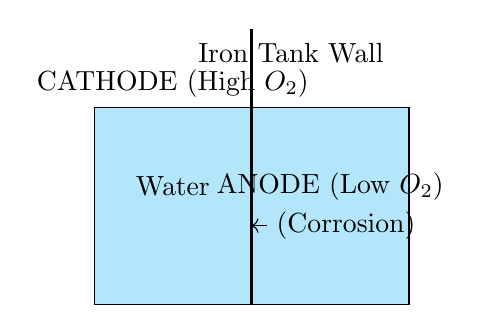
\begin{tikzpicture}
    \draw[fill=cyan!30] (0,0) rectangle (4,2.5);
    \draw[thick] (2,0) -- (2,3.5); \node at (2.5, 3.2) {Iron Tank Wall};
    \draw[dashed] (0, 2.5) -- (4, 2.5); \node at (1, 2.8) {CATHODE (High $O_2$)};
    \node at (1, 1.5) {Water};
    \node at (3, 1.5) {ANODE (Low $O_2$)};
    \node at (3.2, 1) {(Corrosion)};
    \draw[->] (2.2, 1) -- (2, 1);
\end{tikzpicture}
\end{center}
\textbf{Mnemonic:} "Water Air Interface Corrodes" (WAIC)
\end{solutionbox}

\subsection*{Question 4(A)(3) [3 marks]}
\textbf{Explain the working principle of solar cells.}

\begin{solutionbox}
\textbf{Answer}:
\begin{tabular}{|l|l|}
\hline
\textbf{Component} & \textbf{Function} \\ \hline
\textbf{Photovoltaic effect} & Light energy converts to electrical energy \\ \hline
\textbf{p-n junction} & Creates electric field for charge separation \\ \hline
\textbf{Electron-hole pairs} & Generated when photons hit semiconductor \\ \hline
\end{tabular}

\textbf{Process}: Light hits surface $\to$ Electrons excited $\to$ Move across p-n junction $\to$ Current flow in external circuit.

\textbf{Mnemonic:} "Photo Voltaic Junction Creates Current" (PVJCC)
\end{solutionbox}

\section*{Question 4(B) [8 marks]}

\subsection*{Question 4(B)(1) [4 marks]}
\textbf{Demonstrate the function of boundary lubrication with diagram.}

\begin{solutionbox}
\textbf{Answer}:
\textbf{Function}: Used under high load and low speed. A thin molecular layer of lubricant gets adsorbed on metal surfaces, preventing direct metal-to-metal contact.

\textbf{Mechanism}:
\begin{itemize}
    \item Polar ends of lubricant molecules attach to metal.
    \item Hydrocarbon chains stand perpendicular, creating a cushion.
    \item Prevents welding/seizure of surfaces.
\end{itemize}

\textbf{Diagram:}
\begin{center}
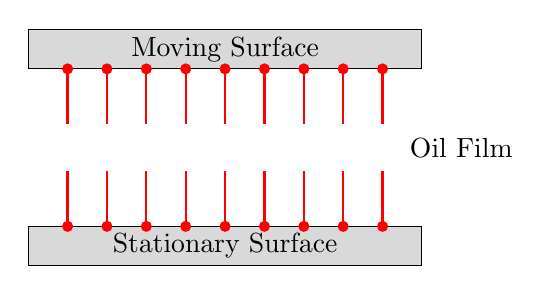
\begin{tikzpicture}
    % Surfaces
    \draw[fill=gray!30] (0,2.5) rectangle (5,3); \node at (2.5, 2.75) {Moving Surface};
    \draw[fill=gray!30] (0,0) rectangle (5,0.5); \node at (2.5, 0.25) {Stationary Surface};
    
    % Lubricant molecules
    \foreach \x in {0.5, 1.0, ..., 4.5} {
        \draw[thick, red] (\x, 0.5) -- (\x, 1.2); \fill[red] (\x, 0.5) circle (2pt);
        \draw[thick, red] (\x, 2.5) -- (\x, 1.8); \fill[red] (\x, 2.5) circle (2pt);
    }
    \node at (5.5, 1.5) {Oil Film};
\end{tikzpicture}
\end{center}
\textbf{Mnemonic:} "Boundary Barriers Prevent Metal Contact" (BBPMC)
\end{solutionbox}

\subsection*{Question 4(B)(2) [4 marks]}
\textbf{Explain how viscosity is measured through redwood viscometer with labelled diagram.}

\begin{solutionbox}
\textbf{Answer}:
\textbf{Principle}: Measures viscosity in "Redwood Seconds" - time taken for 50ml of oil to flow through a standard orifice under gravity.

\textbf{Procedure}:
\begin{enumerate}
    \item Clean and level the instrument.
    \item Fill oil in the cup to pointer level. Heat water bath to desired temp.
    \item Remove ball valve, start stopwatch.
    \item Collect 50ml oil in Kohlrausch flask. Stop watch.
\end{enumerate}
Viscosity = $At - \frac{B}{t}$ (Kinematic viscosity)

\textbf{Diagram:}
\begin{center}
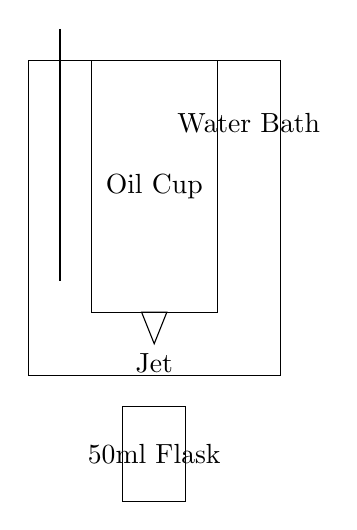
\begin{tikzpicture}[scale=0.8]
    % Outer Bath
    \draw (0,0) rectangle (4,5); \node at (3.5, 4) {Water Bath};
    % Inner Cup
    \draw (1,1) rectangle (3,5); \node at (2, 3) {Oil Cup};
    % Orifice
    \draw (1.8, 1) -- (2.2, 1) -- (2, 0.5) -- cycle; \node at (2, 0.5) [below] {Jet};
    % Flask
    \draw (1.5, -2) rectangle (2.5, -0.5); \node at (2, -1.25) {50ml Flask};
    % Stirrer/Thermometer simplified
    \draw[thick] (0.5, 5.5) -- (0.5, 1.5); 
\end{tikzpicture}
\end{center}
\textbf{Mnemonic:} "Redwood Records Time" (RRT)
\end{solutionbox}

\subsection*{Question 4(B)(3) [4 marks]}
\textbf{Define: Semiconductor, Insulating material, Elastomer, Addition polymerization.}

\begin{solutionbox}
\textbf{Answer}:
\begin{tabular}{|p{4cm}|p{8cm}|}
\hline
\textbf{Term} & \textbf{Definition} \\ \hline
\textbf{Semiconductor} & Material with conductivity between conductor and insulator (e.g., Si, Ge). \\ \hline
\textbf{Insulating material} & Material that resists flow of electric current (e.g., Rubber, Glass). \\ \hline
\textbf{Elastomer} & Polymer with high elasticity, stretches and returns to shape (e.g., Natural Rubber). \\ \hline
\textbf{Addition polymerization} & Monomers join without elimination of by-products (e.g., PE, PVC). \\ \hline
\end{tabular}
\textbf{Mnemonic:} "Semi Insulating Elastic Addition" (SIEA)
\end{solutionbox}

\section*{Question 5(A) [6 marks]}

\subsection*{Question 5(A)(1) [3 marks]}
\textbf{Solve: Calculate the pH and pOH of 0.004 M HCl aqueous solution. (log 4 = 0.6021)}

\begin{solutionbox}
\textbf{Solution}:
\begin{itemize}
    \item HCl is a strong acid, completely ionizes: \ce{HCl -> H+ + Cl-}
    \item $[\ce{H+}] = [\ce{HCl}] = 0.004 \text{ M} = 4 \times 10^{-3} \text{ M}$
    \item $\text{pH} = -\log[\ce{H+}] = -\log(4 \times 10^{-3})$
    \item $\text{pH} = -(\log 4 + \log 10^{-3}) = -(0.6021 - 3) = 2.3979 \approx 2.40$
    \item $\text{pOH} = 14 - \text{pH} = 14 - 2.40 = 11.60$
\end{itemize}
\textbf{Answer}: pH = 2.40, pOH = 11.60
\end{solutionbox}

\subsection*{Question 5(A)(2) [3 marks]}
\textbf{Describe extrinsic semiconductors and it types with examples.}

\begin{solutionbox}
\textbf{Answer}: Extrinsic semiconductors are doped with impurities to increase conductivity.
\begin{tabular}{|l|l|l|l|}
\hline
\textbf{Type} & \textbf{Dopant} & \textbf{Major Carrier} & \textbf{Example} \\ \hline
\textbf{n-type} & Pentavalent (Gr V) (P, As) & Electrons & Si + P \\ \hline
\textbf{p-type} & Trivalent (Gr III) (B, Al) & Holes & Si + B \\ \hline
\end{tabular}
\textbf{Mnemonic:} "n-negative electrons, p-positive holes" (nnep)
\end{solutionbox}

\subsection*{Question 5(A)(3) [3 marks]}
\textbf{Distinguish between thermoplastic polymers and thermosetting polymer (Four points of each)}

\begin{solutionbox}
\textbf{Answer}:
\begin{tabular}{|l|p{5cm}|p{5cm}|}
\hline
\textbf{Property} & \textbf{Thermoplastic} & \textbf{Thermosetting} \\ \hline
\textbf{Structure} & Linear/branched chains & 3D Cross-linked network \\ \hline
\textbf{Heat effect} & Softens on heating, hardens on cooling & Does not soften, chars on heating \\ \hline
\textbf{Reversibility} & Can be remolded (Reversible) & Cannot be remolded (Irreversible) \\ \hline
\textbf{Solubility} & Soluble in organic solvents & Insoluble \\ \hline
\textbf{Example} & PE, PVC, PS & Bakelite, Melamine \\ \hline
\end{tabular}
\textbf{Mnemonic:} "TP=Reversible, TS=Permanent"
\end{solutionbox}

\section*{Question 5(B) [8 marks]}

\subsection*{Question 5(B)(1) [4 marks]}
\textbf{Describe hydrogen bond and its types with examples.}

\begin{solutionbox}
\textbf{Answer}:
\textbf{Definition}: Weak electrostatic attraction between Hydrogen atom covalently bonded to a highly electronegative atom (F, O, N) and another electronegative atom.

\textbf{Types}:
\begin{enumerate}
    \item \textbf{Intermolecular}: Between different molecules (e.g., \ce{H2O}, \ce{HF}, Alcohol). raises BP.
    \item \textbf{Intramolecular}: Within the same molecule (e.g., o-nitrophenol).
\end{enumerate}

\textbf{Diagram (Intermolecular in Water):}
\begin{center}
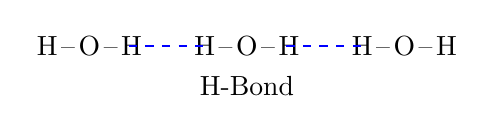
\begin{tikzpicture}
    \node at (0,0) {\ce{H-O-H}};
    \node at (2,0) {\ce{H-O-H}};
    \node at (4,0) {\ce{H-O-H}};
    \draw[dashed, blue, thick] (0.5, 0) -- (1.5, 0);
    \draw[dashed, blue, thick] (2.5, 0) -- (3.5, 0);
    \node at (2, -0.5) {H-Bond};
\end{tikzpicture}
\end{center}
\textbf{Mnemonic:} "Hydrogen Needs FON friends"
\end{solutionbox}

\subsection*{Question 5(B)(2) [4 marks]}
\textbf{Differentiate between Primary cell and Secondary cell. (Four points)}

\begin{solutionbox}
\textbf{Answer}:
\begin{tabular}{|l|p{5cm}|p{5cm}|}
\hline
\textbf{Aspect} & \textbf{Primary Cell} & \textbf{Secondary Cell} \\ \hline
\textbf{Rechargeability} & Not rechargeable & Rechargeable \\ \hline
\textbf{Reaction} & Irreversible & Reversible \\ \hline
\textbf{Life} & Short life & Long life \\ \hline
\textbf{Example} & Dry cell, Daniel cell & Lead-acid, Ni-Cd, Li-ion \\ \hline
\end{tabular}
\textbf{Mnemonic:} "Primary = Permanent, Secondary = Reversible"
\end{solutionbox}

\subsection*{Question 5(B)(3) [4 marks]}
\textbf{Describe construction, working and chemical equations of lead-acid storage cell with a labelled diagram.}

\begin{solutionbox}
\textbf{Answer}:
\textbf{Construction}:
\begin{itemize}
    \item \textbf{Anode}: Spongy Lead (Pb).
    \item \textbf{Cathode}: Lead Dioxide (\ce{PbO2}).
    \item \textbf{Electrolyte}: Dilute \ce{H2SO4} (density 1.25-1.30 g/cc).
\end{itemize}

\textbf{Working (Discharge)}:
\begin{itemize}
    \item Anode: \ce{Pb + SO4^2- -> PbSO4 + 2e-}
    \item Cathode: \ce{PbO2 + 4H+ + SO4^2- + 2e- -> PbSO4 + 2H2O}
    \item Overall: \ce{Pb + PbO2 + 2H2SO4 -> 2PbSO4 + 2H2O + Energy}
\end{itemize}

\textbf{Diagram:}
\begin{center}
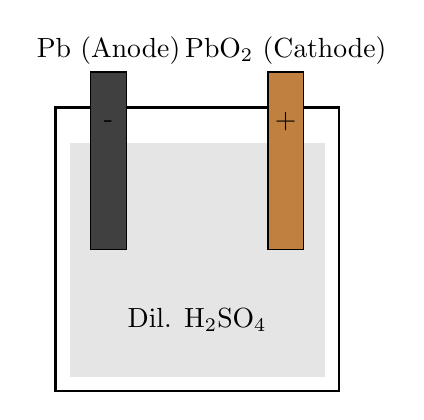
\begin{tikzpicture}[scale=0.9]
    \draw[thick] (0,0) rectangle (4,4);
    \fill[gray!20] (0.2, 0.2) rectangle (3.8, 3.5); \node at (2, 1) {Dil. \ce{H2SO4}};
    
    \draw[fill=darkgray] (0.5, 2) rectangle (1, 4.5); \node at (0.75, 4.8) {Pb (Anode)};
    \draw[fill=brown] (3, 2) rectangle (3.5, 4.5); \node at (3.25, 4.8) {\ce{PbO2} (Cathode)};
    
    \node at (0.75, 3.8) {-}; \node at (3.25, 3.8) {+};
\end{tikzpicture}
\end{center}
\textbf{Mnemonic:} "LASRE = Lead Acid Storage Reversible Energy"
\end{solutionbox}

\end{document}
